\section{Überblick}

asada \bfarmer asd

Version Control: thomas2019pragmatic (data1)

\begin{itemize}
\item Daten Integration per Kommandozeilenbefehl
\item Darstellung der Daten
\item Generieren von ConceptMaps
\item Beispiel-Anwendung: Virtuelle Patienten 
\end{itemize}

Symfony -- Warum?  \cite{potencier2022symfony}

Composer \cite{composer}

PHP Verwendung \cite{w3techs}

Programming Languages Harmful \cite{janssenscan}

Model-View-Controller \cite[Seite 176f]{voorhees2020guide}

\begin{figure}[H]
    \centering
    \setlength{\fboxsep}{10pt}\color{black!20}\fbox{
    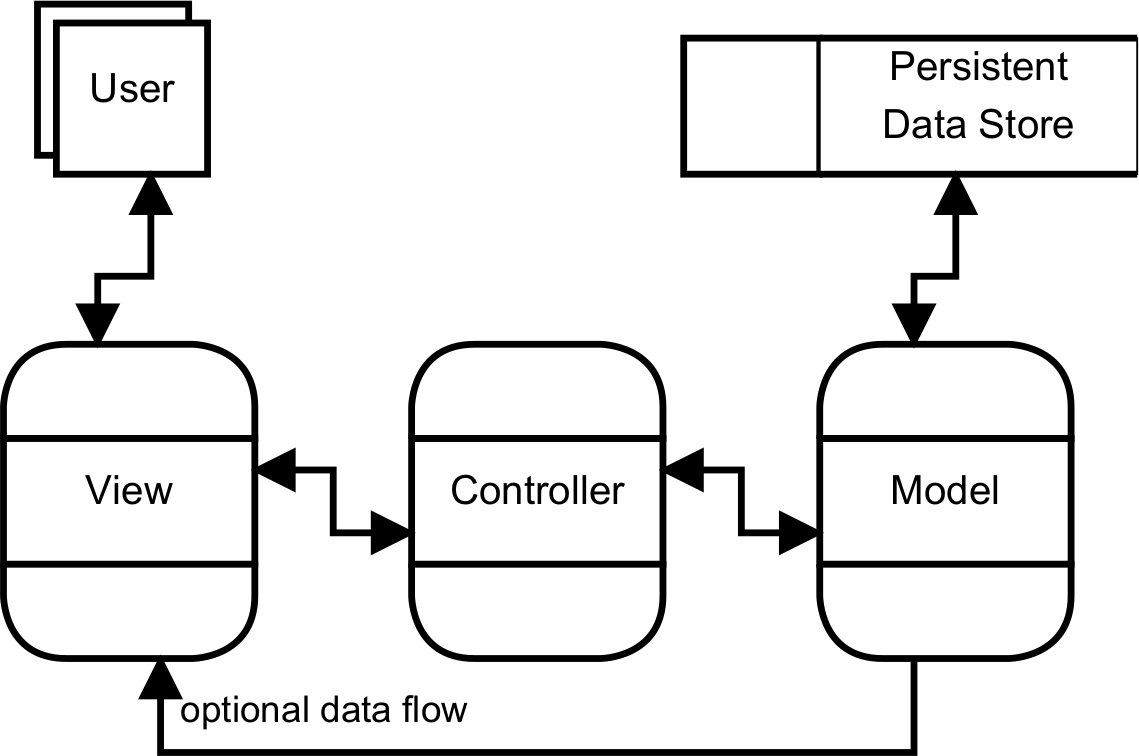
\includegraphics[width=.7\linewidth]{../img/mvc.png}}
    \normalcolor\caption{\cite[Seite 177]{voorhees2020guide}}
\end{figure}

Abstraction and Decoupling -- Orthogonality: thomas2019pragmatic

Symfony \cite{potencier2022symfony}

Dependency Injection \cite{seemann2019dependency}

\subsection{Symfony Komponenten}

Console \cite[Console Commands]{symfony-command}

Http Foundation: Request, Response, StreamedResponse \cite[The HttpFoundation Component]{symfony-http}

HttpClientInterface -- Download \cite[HTTP Client]{symfony-client}

File System \cite[The Filesystem Component]{symfony-file}

UUID \cite[The UID Component]{symfony-uuid}

Controller -- Routing  \cite[Controller]{symfony-controller}

Serializer: XML, CSV, JSON, SQL-Insert \cite[The Serializer Component]{symfony-serializer}

Database \cite[Databases and the Doctrine ORM]{symfony-db}

Templates \cite[Creating and Using Templates]{symfony-templates}

Twig \cite{twig}

\begin{figure}[H]
    \centering
    \setlength{\fboxsep}{10pt}\color{black!20}\fbox{
    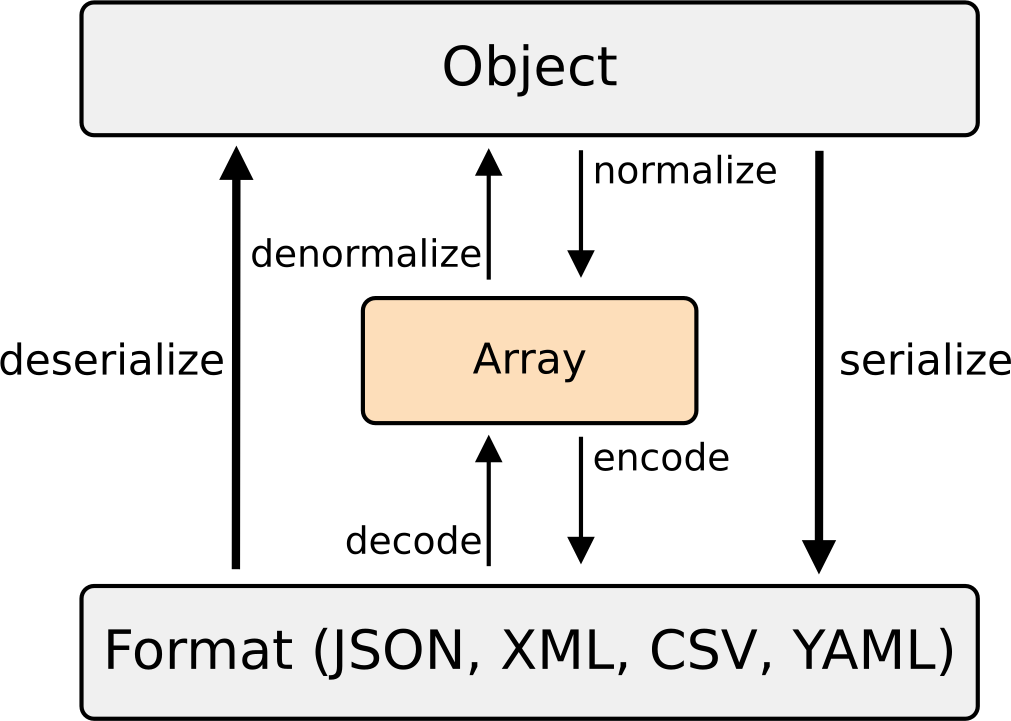
\includegraphics[width=.6\linewidth]{../img/serializer_workflow.png}}
    \normalcolor
\end{figure}

\section{Aufbau des \bfarmer-Projekts}

\subsection{Views}

Templates für HTML-Code. 

\begin{itemize}
\item \texttt{base} \newline Grundvorlage für alle Seiten, also zum Beispiel \texttt{<head>} mit Imports für Stylesheets, Javascript und \texttt{<body>}.
\item \texttt{index} \newline b
\item \texttt{codes} \newline c
\item \texttt{conceptmap} \newline d
\item \texttt{modal} \newline e
\item \texttt{patients} \newline f
\item \texttt{search\_code} \newline g
\item \texttt{umsteiger} \newline h
\item \texttt{umsteiger\_icons} \newline i
\item \texttt{umsteiger\_search} \newline j
\item \texttt{umsteiger\_search\_recursion} \newline k
\item \texttt{umsteiger\_search\_result} \newline l
\end{itemize}

\subsection{Utility}

\begin{itemize}
\item \texttt{Constants} \newline Enthält globale Konstanten und statische Funktionen, die keine Instanziierung einer Klasse benötigen, um zum Beispiel eindeutige Namen für die SQL-Tabellen zu generieren. 
\item \texttt{SqlInsertEncoder} \newline b
\item \texttt{TwigExtension} \newline Erweiterung der Twig-Template Engine, um externe Kode-Links und 
\end{itemize}

\subsection{Repositories}

\begin{itemize}
\item \texttt{BfarmRepository} \newline a
\item \texttt{ConfigRepository} \newline b
\item \texttt{DatabaseRepository} \newline c
\item \texttt{PatientsRepository} \newline d
\end{itemize}

\subsection{Controllers}

\begin{itemize}
\item \texttt{AdminController} \newline a
\item \texttt{CodesController} \newline b
\item \texttt{ConceptMapController} \newline c
\item \texttt{DimdiController} \newline d
\item \texttt{IndexController} \newline e
\item \texttt{PatientsController} \newline f
\item \texttt{UmsteigerController} \newline g
\item \texttt{UmsteigerSearchController} \newline h
\end{itemize}

\subsection{Services}

\begin{itemize}
\item \texttt{ClientService} \newline a
\item \texttt{ConceptMapService} \newline b
\item \texttt{DataService} \newline c
\item \texttt{PatientsService} \newline d
\item \texttt{SetupService} \newline e
\item \texttt{UmsteigerService} \newline f
\end{itemize}

\subsection{Commands}

\begin{itemize}
\item \texttt{BfarmerCommand} \newline a
\item \texttt{TestCommand} \newline b
\end{itemize}

\section{Backend}

\subsection{Setup-XML}

\subsection{Konsole}

\subsection{Datenbank / MySQL / Doctrine}

Database must have collation utf8mb4\_unicode\_ci

\section{Frontend}

HTML \cite{html}, CSS \cite{css}, JavaScript \cite{javascript}

\subsection{Webpack / Node.js}

Webpack \cite{webpack}, NPM \cite{npm}, Node.js \cite{nodejs}

webpack is a static module bundler for modern JavaScript applications

\subsection{Bootstrap}

Bootstrap

Layout, Nav-Tabs, Modal, Icons

\subsection{SCSS}

SASS \cite{sass}: Einfachere Syntax, Variablen, Funktionen

\subsection{Tooltips}

Popper \cite{popperjs}

\section{AJAX}

AJAX \cite{garrett2005ajax}

\begin{figure}[H]
    \centering
    \setlength{\fboxsep}{10pt}\color{black!20}\fbox{
    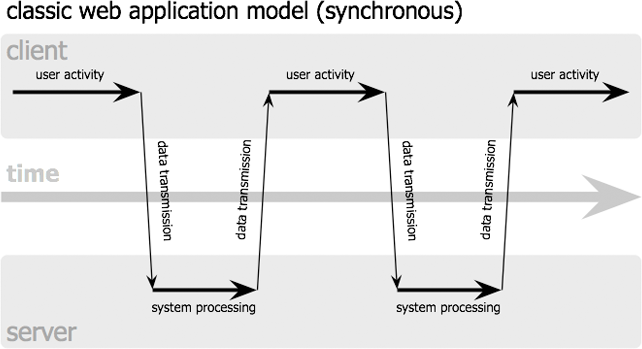
\includegraphics[width=.6\linewidth]{../img/ajax1.png}}
    \normalcolor
\end{figure}

\begin{figure}[H]
    \centering
    \setlength{\fboxsep}{10pt}\color{black!20}\fbox{
    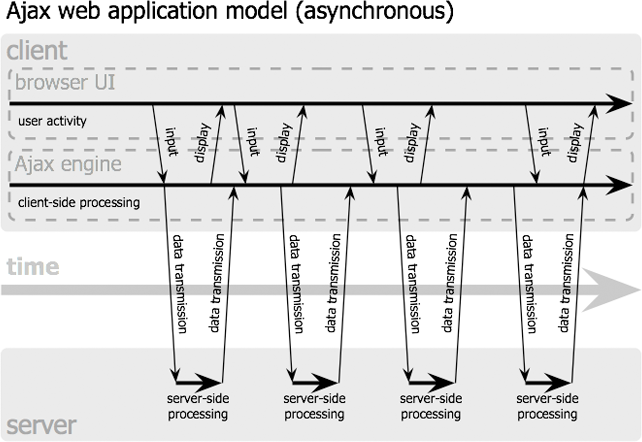
\includegraphics[width=.6\linewidth]{../img/ajax2.png}}
    \normalcolor\caption{\cite{garrett2005ajax}}
\end{figure}


Modal

BfArM/Dimdi Links -- Neuer Tab muss geöffnet werden bevor Skripte ausgeführt werden. 

CSS Flexbox \cite{flexbox-csstricks}

\subsection{Anonyme Funktionen}

Callback

Zum Schreiben der ConceptMap

Data-Preprocessing

InsertEncoder

https://dev.mysql.com/doc/refman/en/insert-optimization.html
